%%%%%%%%%%%%%%%%%%%%%%%%%%%%%%%%%%%55%%
\begin{frame} [plain]
    \frametitle{}
    \Background[1] 
    \begin{center}
    { {\huge 第四章、态和力学量的表象 (8学时)}}
    \end{center}  
    \addtocounter{framenumber}{-1}   
\end{frame}
%%%%%%%%%%%%%%%%%%%%%%%%%%%%%%%%%%

\section{1.矩阵表示}

\begin{frame}
    \frametitle{前情回顾}
    \begin{itemize}
        \Item 波函数 : $$ \Psi(\vec{r},t)$$
        \Item 薛定谔方程 :     
        \begin{equation*}
            i\hbar \frac{\partial }{\partial t} \Psi(\vec{r},t) = (\frac{\hbar^2}{2\mu} \nabla^2 +U(\vec{r})) \Psi(\vec{r},t)
        \end{equation*}
        \Item 力学量算符 :
        $$\left\{ \begin{aligned}
            &\hat{\vec{r}} =\vec{r}  \\
            &\hat{\vec{p}} =-i\hbar(\dfrac{d}{d x}+ \dfrac{d}{d y} + \dfrac{d}{d z}) \\
            &\hat{F}=F(\hat{\vec{r}},\hat{\vec{p}}) \\
        \end{aligned} \right.$$
    \end{itemize}   
    可以发现:所有函数都以位置为自变量!我们称为位置表象
\end{frame} 
%
\begin{frame} 
    \frametitle{表象理论}
    \begin{tcolorbox1}{定义:}
        \begin{itemize}
            \Item 表象:波函数和力学量的具体表示形式,选择一个力学量本征函数系做为基就是选取一种表象
            \Item 表象理论:研究量子力学具体表示形式以及它们之间的相互变换的理论。
        \end{itemize}
    \end{tcolorbox1}
\end{frame} 

\subsection{波函数矩阵表示}

\begin{frame} 
    \frametitle{展开系数}   
    \begin{exampleblock}{命题-1.试证明波函数可用其在任意基上的展开系数构成的矩阵表示}
        $$ \Psi(\vec{r},t)=\sum_n c_n(t) \psi_n(\vec{r})$$ 
        $$ \Psi\Leftrightarrow(c_1,c_2,\cdots)^T $$   
    \end{exampleblock}
    \证 ~对于任意表象Q,若:\\
     本征分立谱: $\psi_n(\vec{r}) \to u_n(\vec{r})$, $c_n \to a_n $
        \begin{equation*}
            a_n(t)=(u_n(\vec{r}), \Psi(\vec{r},t)) 
        \end{equation*}  
    本征连续谱: $\psi_n(\vec{r}) \to u_q(\vec{r})$, $c_n \to a(q) $
        \begin{equation*}
            a(q,t)=(u_q(\vec{r}), \Psi(\vec{r},t)) 
        \end{equation*}  
\end{frame} 

\begin{frame} 
        \frametitle{波函数矩阵表示} 
        \begin{equation*}
            \begin{split} 
                \Psi(\vec{r},t)&=\sum_n a_n(t) u_n(\vec{r}) \\
                &=a_1(t) u_1+ a_2(t) u_2+\cdots+ a_n(t) u_n \\
                &=(u_1,u_2,\cdots,u_n) 
               \begin{pmatrix}
                    a_1(t)\\
                    a_2(t)\\
                    \cdots\\
                    a_n(t)
                \end{pmatrix} \\
                &= (u_1,u_2,\cdots,u_n) (a_1(t),a_2(t),\cdots, a_n(t))^T
            \end{split}  
        \end{equation*}  
        因此,有: $$   \Psi \Leftrightarrow (a_1(t),a_2(t),\cdots, a_n(t))^T \Leftrightarrow {\color{red}  \pmb {\Psi} } $$
\end{frame}

\begin{frame} 
    \frametitle{} 
    $$\begin{matrix}
      ~~  & \text{矢量空间} & \text{希尔伯特空间}\\ \vspace{0.6em}
      \text{基}  & \{\vec{e}_1,\vec{e}_2,\vec{e}_3\}  & \{ u_1,u_2,\cdots,u_n \}\\ \vspace{0.6em}
      \text{正交归一}  & \vec{e}_i \cdot \vec{e}_j=\delta_{ij} & ( u_m, u_n)= \delta_{mn}\\ \vspace{0.6em}
      \text{完备性}  & \vec{P}=\sum\limits_{i=1}^{3} x_i \vec{e}_i &  \Psi=\sum_n a_n(t) u_n \\  \vspace{0.6em}
      \text{投影}  & x_i= \vec{e}_i \cdot \vec{P}  & a_n(t)=( u_m, \Psi) \\ \vspace{0.6em}
      \text{矩阵}  & (x_1, x_2, x_3)^T & (a_1(t), a_2(t), \cdots, a_n(t))^T
      \end{matrix}
      $$
\end{frame}

\begin{frame} 
    \frametitle{实例} 
    \例[2.求动量本征态(平面波)在动量表象中的具体形式(矩阵表示)]{}
    \解~ 动量的本征谱连续,采用公式\\
    $$a(q,t)=(u_q(\vec{r}), \Psi(\vec{r},t)) $$
    取 $$u_q(\vec{r})=\psi_{\vec{p}}(\vec{r})=\frac{1}{(2\pi\hbar)^{3/2}}e^{\frac{i}{\hbar}\vec{p}\cdot \vec{r}}, 
    \qquad \Psi(\vec{r},t))=\frac{1}{(2\pi \hbar)^{3/2}} e^{\frac{i}{\hbar}(\vec p\cdot \vec r -Et)} = 
    \psi_{\vec{p}'}e^{-\frac{i}{\hbar}Et}  $$
\end{frame}

\begin{frame} [allowframebreaks=]
    \frametitle{}
    \begin{equation*}
        \begin{split}
            a(q,t)&=(u_q(\vec{r}), \Psi(\vec{r},t)) \\
            a(p,t)&= (\psi_{\vec{p}}(\vec{r}), \psi_{\vec{p}'}e^{-\frac{i}{\hbar}Et})\\
            &= e^{-\frac{i}{\hbar}Et}(\psi_{\vec{p}}(\vec{r}), \psi_{\vec{p}'})\\
            &= e^{-\frac{i}{\hbar}Et}\delta(\vec{p}-\vec{p}')\\
        \end{split} 
    \end{equation*}
    ~\\
    \Tips~本征态在自身表象中的矩阵表示为$\delta$函数。
\end{frame} 

\begin{frame} [allowframebreaks=]
    \例[3.已知如下波函数是体系的能量本征态,求其基态(n=1)分别在动量和能量表象中的具体形式]
        {$$ \psi_n(x)=\sqrt{\frac{2}{a}} \sin \frac{n\pi}{a}x, \qquad 0<x<a $$}
    \解~ (1)动量的本征谱连续,采用公式\\
    \begin{equation*}
        \begin{split}
            a(q,t)&=(u_q(\vec{r}), \Psi(\vec{r},t)) \\
            a(p)&= (\psi_{p}(x), \psi_1(x))\\
            &= (\frac{1}{\sqrt{2\pi\hbar}}e^{\frac{i}{\hbar}px}, \sqrt{\frac{2}{a}} \sin \frac{\pi}{a}x)
        \end{split} 
    \end{equation*}

    \begin{equation*}
        \begin{split}
          ~~~~~~&= \frac{1}{\sqrt{2\pi\hbar}}\sqrt{\frac{2}{a}} (e^{\frac{i}{\hbar}px},  \sin \frac{\pi}{a}x)\\
            &= \frac{1}{\sqrt{2\pi\hbar}}\sqrt{\frac{2}{a}} \int_0 ^a e^{{\color{red}-}\frac{i}{\hbar}px}\sin \frac{\pi}{a}x) dx\\
            &=\sqrt{\frac{a\pi}{\hbar}} \frac{1+e^{\frac{i}{\hbar}pa}}{\pi^2-p^2a^2/\hbar^2}
        \end{split} 
    \end{equation*}

    (2)能量本征谱分立,采用公式\\
    \begin{equation*}
        \begin{split}
            a_n(t)&=(u_n(\vec{r}), \Psi(\vec{r},t)) \\
            a_{E_n}&=(\psi_n(x), \psi_1(x)) \\
            &=\delta_{1n} \\
        \end{split} 
    \end{equation*}  
\end{frame} 

\subsection{算符的矩阵表示}

\begin{frame}
    \frametitle{算符矩阵表示}    
    \例[4.算符有如下定义式,求其在Q表象的矩阵形式]{
    \begin{equation*}
        \varphi(\vec{r})=F\Psi(\vec{r}) 
    \end{equation*} } 
    \解~ 把两波函数在表象Q中展开(基$u_n(\vec{r})$):\\
    \begin{equation*}
        \begin{split} 
         \sum_m b_m(t)u_m(\vec{r})&= F\sum_m a_m(t)u_m(\vec{r}) \\
         \sum_m b_m(t)u_m(\vec{r})&= \sum_m Fu_m(\vec{r})a_m(t) \\
         \sum_m b_m(t)u_n ^*(\vec{r}) u_m(\vec{r})&= \sum_m u_n ^*(\vec{r}) Fu_m(\vec{r})a_m(t) \\
         \sum_m b_m(t)(u_n (\vec{r}), u_m(\vec{r}))&= \sum_m (u_n (\vec{r}), Fu_m(\vec{r}))a_m(t) \\
        \end{split}  
    \end{equation*} 
\end{frame}

\begin{frame} 
    \begin{equation*}
        \begin{split} 
         \sum_m b_m(t)\delta_{nm}&= \sum_m (u_n (\vec{r}), Fu_m(\vec{r}))a_m(t) \\
         b_n(t)&= \sum_m (u_n (\vec{r}), Fu_m(\vec{r}))a_m(t) \\
         b_n(t)&= \sum_m F_{nm} a_m(t) 
        \end{split}  
    \end{equation*} 
    取遍$n, m$, 得矩阵形式
    $$\begin{pmatrix}
        b_1(t)\\
        b_2(t)\\
        \cdots \\
        b_n(t)
    \end{pmatrix}
    =
    \begin{pmatrix}
       F_{11} & F_{12} & \cdots & F_{1n} \\
       F_{21} & F_{22} & \cdots & F_{2n} \\
       \cdots & \cdots &  \cdots& \cdots\\
        F_{n1} & F_{n2} & \cdots & F_{nn} \\
    \end{pmatrix}
    \begin{pmatrix}
        a_1(t)\\
        a_2(t)\\
        \cdots \\
        a_n(t)
    \end{pmatrix}
    $$
    \Tips~算符矩阵元公式 $$ F_{nm}=(u_n (\vec{r}), Fu_m(\vec{r})) $$
\end{frame} 

\subsection{算符矩阵的厄密性}

\begin{frame} 
    \frametitle{算符矩阵性质} 
    \begin{enumerate}
    \Item  力学量算符的矩阵是厄密矩阵 
    \Item  力学量算符的矩阵,对角元都是实数
    \Item  力学量算符在自身表象是对角矩阵,对角元素就是算符的本征值
    \end{enumerate}
\end{frame}

\begin{frame} 
    \begin{tcolorbox1}{厄密矩阵定义:}
        \begin{itemize}
        \Item 对于矩阵F,其共轭矩阵为:$F^{\dagger } =(F_{nm} ^*)^T$
        \Item 如果有 $F= F^{\dagger }$, 称F为厄密矩阵
        \end{itemize}
    \Tips~厄密矩阵的矩阵元有特点 $$  F_{nm}^* = F_{mn}  $$
    \end{tcolorbox1}
\end{frame}

\begin{frame} 
    \frametitle{} 
    \例[5.指出下列矩阵,哪些是厄密矩阵]{}
    $$\begin{matrix}
        \begin{pmatrix}
            a & 0 & 0 & 0 \\
            0 & b & 0 & 0 \\
            0 & 0 & c & 0\\
            0 & 0 & 0 & 0 \\
         \end{pmatrix} 
         &  
         \begin{pmatrix}
            a & 1 & 0 & 0 \\
            2 & b & 0 & 0 \\
            0 & 0 & c & 0\\
            0 & 0 & 0 & 0 \\
         \end{pmatrix} 
         & 
         \begin{pmatrix}
            a & 1 & 0 & 0 \\
            1 & b & 0 & 0 \\
            0 & 0 & c & 0 \\
            0 & 0 & 0 & 0 \\
         \end{pmatrix} 
         \\ \vspace{0.6em}
         \begin{pmatrix}
            a & 1 & 0 & 0 \\
            -1 & b & 0 & 0 \\
            0 & 0 & c & 0 \\
            0 & 0 & 0 & 0 \\
         \end{pmatrix} 
         &     
        \begin{pmatrix}
            a & i & 0 & 0 \\
            i & b & 0 & 0 \\
            0 & 0 & c & 0 \\
            0 & 0 & 0 & 0 \\
        \end{pmatrix} 
         &   
         \begin{pmatrix}
            a & -i & 0 & 0 \\
            i & b & 0 & 0 \\
            0 & 0 & c & 0 \\
            0 & 0 & 0 & 0 \\
         \end{pmatrix} 
    \end{matrix}
        $$
\end{frame}


\begin{frame}
    \frametitle{性质1:}
    \例[6.试证明力学量算符的矩阵表示都是厄密矩阵]{}
    \证~ 
    \begin{equation*}
        \begin{split}
            F_{nm}&=(u_n (\vec{r}), Fu_m(\vec{r}))\\
            &=(Fu_n (\vec{r}), u_m(\vec{r}))\\
            &=(u_m(\vec{r}), Fu_n (\vec{r}))^*\\
            &=F_{mn}^*\\
        \end{split} 
    \end{equation*}
    证毕!
\end{frame}

\begin{frame}
    \frametitle{性质2:}
    \例[7.试证明力学量算符的矩阵表示,对角元都是实数]{}
    \证~ 
    \begin{equation*}
        \begin{split}
            F_{nm}&=F_{mn}^*\\
            F_{nn}&=F_{nn}^*\\
        \end{split} 
    \end{equation*}
    即:对角元都是实数。 \\
    证毕!
\end{frame}

\begin{frame}
    \frametitle{性质3:}
    \例[8.试证明力学量算符的矩阵表示,在自身表象中是对角矩阵]{}
    \证~ 
    \begin{equation*}
        \begin{split}
            F_{nm}&=(u_n (\vec{r}), Fu_m(\vec{r}))\\
            &=(u_n (\vec{r}), f_nu_m(\vec{r}))\\
            &=f_n(u_n (\vec{r}), u_m(\vec{r}))\\
            &=f_n\delta_{mn}\\
        \end{split} 
    \end{equation*}
    即:(1)非对角元都是0,是对称阵。(2)对角元就是本征值\\
    证毕!
\end{frame}

\begin{frame} [allowframebreaks=]
    \begin{tcolorbox2}{对角化的物理意义}
        \begin{itemize}
            \Item 力学量算符的表示一般不是对称阵(不在自身表象)
            \Item 在数学上做矩阵对角化,使其成为对角阵 (在自身表象)
            \Item 对角化完成从任意表象回到自身表象的过程
            \Item 对角元就是本征值(解本征方程求本征值)
        \end{itemize}  
    \end{tcolorbox2}
\end{frame}

\begin{frame} 
    \frametitle{}
    \begin{exampleblock}{课堂作业:}
    取Q表象为动量表象,试求位置算符$\hat{x}$、动量算符$\hat{p}_x$ 的具体形式。
    \end{exampleblock}
\end{frame} 

\begin{frame} 
    \frametitle{}
    \begin{tcolorbox2}{课堂讨论}
    已知波函数取如下形式:$$\psi(x)=\dfrac{1}{\sqrt{2}}u_1(x)+\dfrac{1}{2}u_2(x)+\dfrac{1}{2}u_3(x)$$
    其系数矩阵为$$\begin{pmatrix}
            \dfrac{1}{\sqrt{2}}\\
            \dfrac{1}{2}\\
            \dfrac{1}{2}
            \end{pmatrix}$$
    \begin{enumerate}
        \Item  此系数矩阵是波函数在位置表象的矩阵表示吗?
        \Item  此系数矩阵是波函数在能量表象的矩阵表示的条件是什么?  
    \end{enumerate}
    \end{tcolorbox2}
\end{frame} 

%%%%%%%%%%%%%%%%%%%%%%%%%%%%%%%%%%%%%%%%%%%%%%%%%%%%%%%%%%%%%%%%%%%
\begin{frame}
    \frametitle{课外作业}
    \begin{enumerate}
        \item 求动量表象中的位置算符和动量算符的具体形式
        \item 求动量表象中位置算符的本征值和本征函数
    \end{enumerate}
\end{frame}
%%%%%%%%%%%%%%%%%%%%%%%%%%%%%%%%%%%%%%%%%%%%%%%%%%%%%%%%%%%%%%%%%%%


\subsection{公式的矩阵表示}

\begin{frame}
%    \frametitle{前情回顾}
%   \begin{itemize}
%      \Item 波函数矩阵表示 :$ a_n(t)=(u_n(\vec{r}), \Psi(\vec{r},t)) $ 
%      \Item 力学量算符矩阵表示 : $ F_{nm} = (u_n (\vec{r}), Fu_m(\vec{r})) $   
%      \Item 公式的矩阵表示:$\cdots$
%   \end{itemize}
\end{frame} 

\begin{frame} 
    \frametitle{}
    \begin{tcolorbox2}{量子力学常用公式}
        \begin{itemize}
            \Item 平均值公式
            \Item 归一化公式
            \Item 本征方程
            \Item 薛定谔方程
            \Item 运动方程
        \end{itemize}   
    \end{tcolorbox2}
\end{frame} 

\begin{frame} 
    \frametitle{平均值公式}
    \例[1、求平均值公式在Q表象中的具体形式(矩阵表示)] {
        $$ \bar{F}=\int \Psi^* (\vec{r},t) F \Psi(\vec{r},t) d\tau $$}
    \解~ 
    \begin{equation*}
        \begin{split}
            \bar{F}&=(\Psi(\vec{r},t), F\Psi(\vec{r},t)) \\
            &= (\sum_n a_n(t) u_n(\vec{r}), \sum_m a_m(t) F u_m(\vec{r}))\\
            &= \sum_{n,m} a_n ^*(t) (u_n(\vec{r}), F u_m(\vec{r})) a_m(t)\\
            &= \sum_{n,m} a_n ^*(t) F_{nm} a_m(t)\\
        \end{split} 
    \end{equation*}
\end{frame}

\begin{frame} 
    取遍$n, m$, 得到如下矩阵形式\\
    $$\bar{F} =(a_1 ^*(t), a_2 ^*(t),\cdots,a_n^*(t) )
    \begin{pmatrix}
       F_{11} & F_{12} & \cdots & F_{1n} \\
       F_{21} & F_{22} & \cdots & F_{2n} \\
       \cdots & \cdots &  \cdots& \cdots\\
        F_{n1} & F_{n2} & \cdots & F_{nn} \\
    \end{pmatrix}
    \begin{pmatrix}
        a_1(t)\\
        a_2(t)\\
        \cdots \\
        a_n(t)
    \end{pmatrix}
    $$ \vspace{1.0em} 
    $$ \large \color{red} \bar{F} = \pmb {\Psi} ^{\dagger } \pmb {F} \pmb {\Psi} $$
\end{frame}

\begin{frame} 
    在自身表象中,有:
    $$\bar{F} =(a_1 ^*(t), a_2 ^*(t),\cdots,a_n^*(t) )
    \begin{pmatrix}
       f_1 & 0 & \cdots & 0 \\
       0& f_2 & \cdots & 0 \\
       \cdots & \cdots &  \cdots& \cdots\\
        0 & 0 & \cdots & f_n \\
    \end{pmatrix}
    \begin{pmatrix}
        a_1(t)\\
        a_2(t)\\
        \cdots \\
        a_n(t)
    \end{pmatrix}
    $$
    \vspace{1.0em} 
    $$ \large \color{red} \bar{F} = \sum_n a_n^*(t) a_n(t) f_n= \sum_n |a_n(t)|^2 f_n $$
\end{frame}

\begin{frame} 
    \frametitle{归一化公式}
    \例[2、求归一化公式在Q表象中的具体形式(矩阵表示)]
        {$$ \int \Psi^* (\vec{r},t) \Psi(\vec{r},t) d\tau =1 $$}
    \解~ 
    \begin{equation*}
        \begin{split}
            1 &=(\Psi(\vec{r},t), \Psi(\vec{r},t)) \\
            &= (\sum_n a_n(t) u_n(\vec{r}), \sum_m a_m(t) u_m(\vec{r}))\\
            &= \sum_{n,m} a_n ^*(t) (u_n(\vec{r}), u_m(\vec{r})) a_m(t)\\
            &= \sum_{n,m} a_n ^*(t) \delta_{nm} a_m(t)\\
        \end{split} 
    \end{equation*}
\end{frame}


\begin{frame} 
    $$  \sum_{n} a_n ^*(t) a_n(t) =1 $$
    取遍$n$, 得到如下矩阵形式\\
    $$ (a_1 ^*(t), a_2 ^*(t),\cdots,a_n^*(t) )
    \begin{pmatrix}
        a_1(t)\\
        a_2(t)\\
        \cdots \\
        a_n(t)
    \end{pmatrix}
    =1 $$ \vspace{1.0em} 
    $$ \large \color{red} \pmb {\Psi} ^{\dagger } \pmb {\Psi} =1 $$

\end{frame}

\begin{frame} 
    \frametitle{本征方程}
    \例[3、求本征方程在Q表象中的具体形式(矩阵表示)]
        {$$ F\psi_n (\vec{r}) =f \psi_n (\vec{r})$$}
    \解~ 
    \begin{equation*}
        \begin{split}
            F\psi_m (\vec{r}) &=f \psi_m \\
            \psi_n ^*  F\psi_m &=\psi_n ^* f \psi_m\\
            (\psi_n, F\psi_m )&=(\psi_n, f \psi_m)\\
            (\psi_n, F\psi_m )&=f(\psi_n, \psi_m)\\
            F_{nm} &=f \delta_{nm}
        \end{split} 
    \end{equation*}
\end{frame}

\begin{frame} 
    $$ \sum_n (F_{nm} -f \delta_{nm})a_n=0 $$
    取遍$n,m$, 得矩阵形式\\            
    $$\begin{pmatrix}
        F_{11}-f & F_{12} & \cdots & F_{1n} \\
        F_{21} & F_{22}-f & \cdots & F_{2n} \\
        \cdots & \cdots &  \cdots& \cdots\\
         F_{n1} & F_{n2} & \cdots & F_{nn}-f \\
     \end{pmatrix}
     \begin{pmatrix}
         a_1(t)\\
         a_2(t)\\
         \cdots \\
         a_n(t)
     \end{pmatrix}
     =0 \qquad (1)$$
     $$ \color{red} (\pmb F -f \pmb I) \pmb \Psi =0 $$

    有解条件,系数行列式等于零!
\end{frame}

\begin{frame} 
    得久期方程:
    $$\begin{vmatrix}
        F_{11}-f & F_{12} & \cdots & F_{1n} \\
        F_{21} & F_{22}-f & \cdots & F_{2n} \\
        \cdots & \cdots &  \cdots& \cdots\\
         F_{n1} & F_{n2} & \cdots & F_{nn}-f \\
     \end{vmatrix} 
     =0 \qquad (2) $$
     解久期方程, 得本征谱{$f_1,f_2,\cdots, f_n $}\\
     依次把$f_i$ 代回方程(1),解得第i个本征函数。本征方程得解\\
     矩阵化使本征方程从微分方程变为代数方程!
\end{frame}

\begin{frame} 
    \例[4、已知算符在Q表象中的矩阵形式如下,求本征值和归一化本征函数,并将矩阵对角化。]
        {$$ L_x= \frac{\hbar}{\sqrt{2}}
        \begin{pmatrix}
            0 & 1 & 0  \\
            1 & 0 & 1  \\
            0 & 1 & 0 \\
         \end{pmatrix} $$
        }
    可选方案:
    \begin{itemize}
        \done 解久期方程,得本征值,然后代入方程(1),得本征函数 ,再直接写出对角阵 
        \todo 直接从数学上对角化,对角元就是本征值,然后代入方程(1),得本征函数。
     \end{itemize}
\end{frame}

\begin{frame} 
    \解~第一步:解久期方程求本征值
    $$\frac{\hbar}{\sqrt{2}}
    \begin{vmatrix}
       0-f & 1 & 0  \\
       1 & 0-f & 1  \\
       0 & 1 & 0-f \\
    \end{vmatrix} 
    =0 \qquad (2) $$
   $$ -f^3+2f=0 $$
   $$ f_1=\sqrt{2}, f_2=0, f_3=-\sqrt{2} $$
   注意:这只是
   $$\begin{pmatrix}
       0 & 1 & 0  \\
       1 & 0 & 1  \\
       0 & 1 & 0 \\
    \end{pmatrix} $$
    的本征值,$L_x$的本征值为 $\lambda_i=\dfrac{\hbar}{\sqrt{2}} f_i$,即 $ \hbar, 0, -\hbar$
\end{frame}

\begin{frame} 
    第二步:把$f_i$ 代回方程(1)求本征函数
    $$\begin{pmatrix}
        0-f & 1 & 0  \\
        1 & 0-f & 1  \\
        0 & 1 & 0-f \\
     \end{pmatrix} 
     \begin{pmatrix}
         a_1\\
         a_2\\
         a_3
     \end{pmatrix}
     =0 \qquad (1)$$

     $$\begin{matrix}
       f_1=\sqrt{2} & f_2=0  &  f_3=-\sqrt{2}\\
    \begin{pmatrix}
        1/\sqrt{2}a_2\\
        a_2\\
        1/\sqrt{2}a_2
    \end{pmatrix}  
    = 1/\sqrt{2}a_2 \begin{pmatrix}
        1\\
        \sqrt{2}\\
        1
        \end{pmatrix} 
    & 
    \begin{pmatrix}
        a_1\\
        0\\
        a_1
    \end{pmatrix}  
    =  a_1 \begin{pmatrix}
        1\\
        0\\
        1
    \end{pmatrix}
    &
    \begin{pmatrix}
        -1/\sqrt{2}a_2\\
        a_2\\
        -1/\sqrt{2}a_2
    \end{pmatrix} 
    = 1/\sqrt{2}a_2 \begin{pmatrix}
        -1\\
        \sqrt{2}\\
        -1
    \end{pmatrix} 
    \end{matrix}$$           
\end{frame}


\begin{frame} 
    代入归一化公式, $$ \pmb {\Psi} ^{\dagger } \pmb {\Psi} =1 $$
    $$\begin{matrix}
    f_1=\sqrt{2} & f_2=0  &  f_3=-\sqrt{2}\\
    \dfrac{1}{2} a_2 ^2 (1, \sqrt{2}, 1)
    \begin{pmatrix}
    1\\
    {\sqrt{2}}\\
    1
    \end{pmatrix} 
    =1 
    & 
    a_1 ^2 (1, 0, 1)
    \begin{pmatrix}
     1\\
     0\\
     1
    \end{pmatrix} 
    =1 
     &
     \dfrac{1}{2} a_2 ^2 (-1, \sqrt{2}, -1)
    \begin{pmatrix}
     -1\\
     {\sqrt{2}}\\
     -1
    \end{pmatrix} 
    =1 \\
    a_2= \dfrac{1}{\sqrt{2}} &  a_1= \dfrac{1}{\sqrt{2}} &   a_2=\dfrac{1}{\sqrt{2}} 
    \\
    \psi_1=\dfrac{1}{2}
    \begin{pmatrix}
    1\\
    \sqrt{2}\\
    1
    \end{pmatrix}  
    & 
    \psi_2=\dfrac{1}{\sqrt{2}}
    \begin{pmatrix}
    1\\
    0\\
    1
    \end{pmatrix}  
    &
    \psi_3=\dfrac{1}{2}
    \begin{pmatrix}
    -1\\
    \sqrt{2}\\
    -1
    \end{pmatrix}  
    \end{matrix}$$   
\end{frame}

\begin{frame} 
    第三步:写出对角阵:
    $$ L_x= \frac{\hbar}{\sqrt{2}}
        \begin{pmatrix}
            0 & 1 & 0  \\
            1 & 0 & 1  \\
            0 & 1 & 0 \\
         \end{pmatrix} 
    = 
    \begin{pmatrix}
        \hbar & 0 & 0  \\
        0 & 0 &   0\\
        0 & 0 & -\hbar \\
     \end{pmatrix} 
    $$
\end{frame}

\begin{frame} 
    \frametitle{薛定谔方程}
    \例[5、求薛定谔方程在Q表象中的具体形式(矩阵表示)]
        {$$ i\hbar \frac{\partial}{\partial t }\psi (\vec{r},t) =H\psi (\vec{r},t)$$}
    \解~ 波函数在Q表象展开
    \begin{equation*}
        \begin{split}
            i\hbar \frac{\partial}{\partial t }\sum_n a_n(t) u_n(\vec{r})  &=H\sum_n a_n(t) u_n(\vec{r}) \\
            u_m ^* (\vec{r}) i\hbar \frac{\partial}{\partial t }\sum_n a_n(t) u_n(\vec{r})  &=u_m ^* (\vec{r})H\sum_n a_n(t) u_n(\vec{r}) \\
            i\hbar \frac{\partial}{\partial t }u_m ^* (\vec{r}) \sum_n a_n(t) u_n(\vec{r})  &=u_m ^* (\vec{r})\sum_n a_n(t) Hu_n(\vec{r}) \\      
        \end{split} 
    \end{equation*}
\end{frame}

\begin{frame} 
    \begin{equation*}
        \begin{split}
            i\hbar \frac{\partial}{\partial t }(u_m (\vec{r}), \sum_n a_n(t) u_n(\vec{r}) ) &=(u_m (\vec{r}), \sum_n a_n(t) Hu_n(\vec{r})) \\
            i\hbar \frac{\partial}{\partial t }\sum_n a_n(t)(u_m (\vec{r}),  u_n(\vec{r}) ) &=\sum_n (u_m (\vec{r}),  Hu_n(\vec{r}))a_n(t) \\
            i\hbar \frac{\partial}{\partial t }\sum_n a_n(t)\delta_{mn} &=\sum_n  H_{mn} a_n(t) \\
            i\hbar \frac{\partial}{\partial t } a_n(t) &=\sum_n H_{mn} a_n(t)  \\
        \end{split} 
    \end{equation*}
\end{frame}

\begin{frame} 
    取遍$n,m$, 得矩阵形式\\ 
    $$i\hbar \frac{\partial}{\partial t }  
    \begin{pmatrix}
        a_1(t)\\
        a_2(t)\\
        \cdots \\
        a_n(t)
    \end{pmatrix}
    =         
    \begin{pmatrix}
        H_{11} & H_{12} & \cdots & H_{1n} \\
        H_{21} & H_{22} & \cdots & H_{2n} \\
        \cdots & \cdots &  \cdots& \cdots\\
        H_{n1} & F_{n2} & \cdots & H_{nn} \\
     \end{pmatrix}
     \begin{pmatrix}
         a_1(t)\\
         a_2(t)\\
         \cdots \\
         a_n(t)
     \end{pmatrix}
    $$ \vspace{0.6em }
    $$\color{red} i\hbar \frac{\partial}{\partial t }  \pmb \Psi = \pmb H  \pmb \Psi $$
\end{frame}

\begin{frame} 
    \frametitle{算符运动方程}
    \例[6、求运动方程在Q表象中的具体形式(矩阵表示)]
        {$$ \frac{d\overline{F}}{dt}=\overline{\frac{\partial F }{\partial t}}  +\frac{1}{i\hbar} \overline{[F,H]}$$}
    \解~波函数在Q表象展
    \begin{equation*}
        \begin{split}
            \frac{d(\psi,F \psi )}{dt} &=(\psi,\frac{\partial F }{\partial t} \psi)  +\frac{1}{i\hbar}  ( \psi,[F,H]\psi) \\
            \frac{d(\sum_m a_m u_m,F \sum_n a_n u_n )}{dt} &=(\sum_m a_m u_m,\frac{\partial F }{\partial t} \sum_n a_n u_n) \\  
            &+\frac{1}{i\hbar}  (\sum_m a_m u_m,[F,H]\sum_n a_n u_n)  \\    
        \end{split} 
    \end{equation*}
\end{frame}

\begin{frame} 
    \begin{equation*}
        \begin{split}
            \frac{d\sum_{mn}a_m ^* (u_m,Fu_n )a_n}{dt} &=\sum_{mn} a_m ^*  (u_m,\frac{\partial F }{\partial t} u_n)a_n \\  
            &+\frac{1}{i\hbar} \sum_{mn} a_m ^*  ( u_m,[F,H] u_n)a_n  \\  
            \frac{d\sum_{mn}a_m ^* F_{mn}a_n}{dt} &=\sum_{mn} a_m ^*  \frac{\partial F_{mn} }{\partial t}a_n \\  
            &+\frac{1}{i\hbar} \sum_{mn} a_m ^* [F_{mn},H_{mn}]a_n  \\       
        \end{split} 
    \end{equation*}
\end{frame}

\begin{frame} 
    取遍$n,m$, 得矩阵形式
    \begin{equation*}
        \begin{split} 
            \frac{d \pmb \Psi^{\dagger } \pmb F \pmb \Psi}{dt} &=\pmb \Psi^{\dagger } \frac{\partial \pmb F }{\partial t} \pmb \Psi +\frac{1}{i\hbar} \pmb \Psi^{\dagger } [\pmb F, \pmb H] \pmb \Psi \\ \vspace{0.6em}  
           \color{red} \frac{d \overline{\pmb F}}{dt} & \color{red} =\overline{\frac{\partial \pmb F }{\partial t}} +\frac{1}{i\hbar} \overline{ [\pmb F,\pmb H]} \\      
        \end{split} 
    \end{equation*}
\end{frame}

%%%%%%%%%%%%%%%%%%%%%%%%%%%%%%%%%%%%%%%%%%%%%%%%%%%%%%%%%%%%%%%%%%%
\begin{frame}
    \frametitle{课外作业}
    \begin{enumerate}
        \item 取Q表象为动量表象,试求平均值公式和薛定谔方程的具体形式。
        \item 在$L_z$表象中,$L_x$ 和 $L_y$的矩阵表示如下,求它们的本征值和归一化本征矢 \\
        \[L_x= \frac{\hbar}{\sqrt{2}}\begin{bmatrix}
            0 & 1 & 0 \\
            1 & 0 & 1 \\
            0 & 1 & 0
        \end{bmatrix}, \quad L_y= \frac{\hbar}{\sqrt{2}}\begin{bmatrix}
            0 & -i & 0 \\
            i & 0 & -i \\
            0 & i & 0
        \end{bmatrix} \]
    \end{enumerate}
\end{frame}
%%%%%%%%%%%%%%%%%%%%%%%%%%%%%%%%%%%%%%%%%%%%%%%%%%%%%%%%%%%%%%%%%%%



\section{2.幺正变换}

\begin{frame}
    \frametitle{前情回顾}
    \begin{itemize}
       \done 波函数,力学量算符,公式在Q表象下的矩阵表示 
       \todo 表象变换
    \end{itemize}
\end{frame} 

\subsection{幺正变换的定义}

\begin{frame} 
    \frametitle{}
    \begin{tcolorbox1}{幺正矩阵和厄密矩阵}
        \begin{enumerate}
            \Item F的逆算符$F^{-1}F=FF^{-1}=I$, $$F\Psi=\psi, \qquad \Psi=F^{-1}\psi$$  
            \Item F的共轭算符(称伴算符) $F^{\dagger}=(F_{nm} ^*)^T$, $$ (\psi, F\Psi), \qquad (F^{\dagger}\psi, \Psi)$$
            如果$F^{\dagger } =F$,称F为{\color{red}厄密算符(矩阵)}, 
            判定: $F_{mn}=F_{nm} ^*$; 
            \\ 如果$ F^{\dagger }=F^{-1}$,称F为{\color{red} 幺正算符(矩阵)}, 判定:$F^{\dagger} F= FF^{\dagger}=I$
        \end{enumerate}       
    \end{tcolorbox1}
\end{frame}

\begin{frame} 
    \frametitle{}
    \begin{tcolorbox1}{幺正变换的定义}
    通过幺正矩阵联系起来的两矩阵之间的变换,称为幺正变换。
    \end{tcolorbox1}
\end{frame}

\begin{frame}     
    \例[1. 试证明二维平面矢量绕原点的旋转变换是幺正变换]{}
    \begin{wrapfigure} {r} {0.30\textwidth} %;图在右
        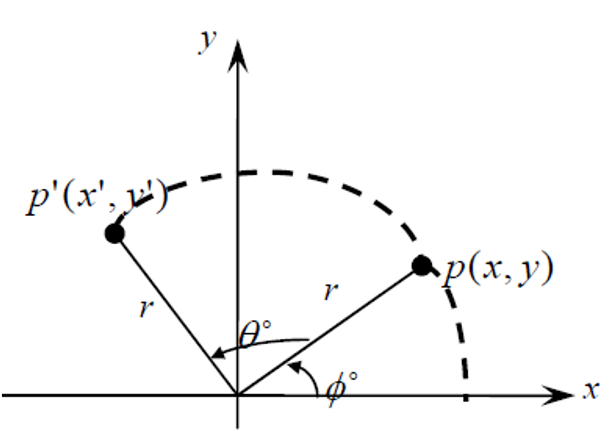
\includegraphics[width=0.29\textwidth]{figs/transf1.png}   
    \end{wrapfigure}
    \证~
    $\left\{\begin{matrix}
        x'=x\cos\theta -y\sin\theta\\
        y'=x\sin\theta+y\cos\theta
    \end{matrix}\right.$ \quad
    $\begin{bmatrix}
        x' \\
        y'
    \end{bmatrix}
    =
    \begin{bmatrix}
        \cos\theta & -\sin\theta\\
        \sin\theta & \cos\theta
    \end{bmatrix}
    \begin{bmatrix}
        x \\
        y
    \end{bmatrix}$\\
    $$ R_\theta=
    \begin{bmatrix}
        \cos\theta &-\sin\theta\\
        \sin\theta &\cos\theta
    \end{bmatrix} ,\qquad
    R_\theta ^{\dagger}=
    \begin{bmatrix}
        \cos\theta &\sin\theta\\
        -\sin\theta &\cos\theta
    \end{bmatrix} $$
    $$ R_\theta  R_\theta ^{\dagger} = R_\theta ^{\dagger} R_\theta=  
    \begin{bmatrix}
        \cos\theta &-\sin\theta\\
        \sin\theta &\cos\theta
    \end{bmatrix}
    \begin{bmatrix}
        \cos\theta &\sin\theta\\
        -\sin\theta &\cos\theta
    \end{bmatrix}
    =I
    $$
    证毕!
\end{frame}

\subsection{量子力学中的三种基本变换}

\begin{frame} 
    \frametitle{基矢变换}
    \例[2.试证明量子力学不同表象基组之间的变换是幺正变换]{}  
    \证~ 设A的基组为$\psi_\alpha$ B的基组为 $\varphi_n$, A归一化公式中把波函数在B展开: 
    \begin{equation*}
        \begin{split}
            \delta_{\alpha\beta} &= (\psi_\alpha, \psi_\beta) \\
            &= (\sum_n S_{n\alpha} \varphi_n, \sum_m S_{m\beta} \varphi_m)\\
            &= \sum_{nm} S_{n\alpha} ^* S_{m\beta}(\varphi_n, \varphi_m)\\
            &= \sum_{nm} S_{n\alpha} ^* S_{m\beta}\delta_{nm}\\
            &= \sum_{n} S_{n\alpha} ^* S_{n\beta} = \sum_{n} S^{\dagger } _{\alpha n} S_{n\beta}
        \end{split} 
    \end{equation*}
\end{frame}

\begin{frame} 
    B归一化公式也可在A展开: 
    \begin{equation*}
        \begin{split}
            \sum_{\alpha} S_{n\alpha}  S^{\dagger } _{\alpha m}&=\sum_{\alpha} S_{n\alpha}  S_{m \alpha} ^* \\
            &=\sum_{\alpha} (\varphi_n, \psi_\alpha) (\varphi_m, \psi_\alpha)^* \\
            &=\sum_{\alpha} (\psi_\alpha,\varphi_n)^* (\psi_\alpha,\varphi_m) \\
            &=\sum_{\alpha\beta} (\psi_\alpha,\varphi_n)^* (\psi_\beta,\varphi_m) \delta_{\alpha\beta} \\
            &=\sum_{\alpha\beta} S_{\alpha n}^*  S_{\beta m} (\psi_\alpha,\psi_\beta)\\
            &= (\sum_{\alpha} S_{\alpha n}\psi_\alpha,\sum_{\beta} S_{\beta m}\psi_\beta)\\
            &= (\varphi_n,\varphi_m) =\delta_{nm} 
        \end{split} 
    \end{equation*}
\end{frame}

\begin{frame} 
    因此,我们有:
    \begin{equation*}
        \begin{split}
            \sum_{\alpha} S_{n\alpha}   S^{\dagger } _{\alpha m} &=\delta_{nm} \\
            \sum_{n} S^{\dagger } _{\alpha n} S_{n\beta}&=\delta_{\alpha\beta}
        \end{split} 
    \end{equation*}
    即:$$ S^{\dagger }S=SS^{\dagger } =I$$ 
    证毕! \\

    注意到: $ S_{n\alpha} = (e_n, e_\alpha)= (e_{(B)}, e_{(A)})$ \\
    得变换公式: $$ \color{red} u_{(B)}= S^{\dagger} u_ {(A)}$$
\end{frame}


\begin{frame} {波函数变换}
    \例[3.试证明同一波函数在两不同表象中的矩阵之间的变换是幺正变换]{}  
    \证~ 设A的基组为$\psi_\alpha$ B的基组为 $\varphi_n$\\
    波函数$\Psi$在A表象和B表象中分别展开:
    \begin{equation*}
        \begin{split}
            \sum_\alpha a_\alpha \psi_\alpha &= \sum_n b_n \varphi_n \\
            \sum_\alpha a_\alpha \psi_\beta ^* \psi_\alpha &= \sum_n b_n \psi_\beta ^* \varphi_n \\
            \sum_\alpha a_\alpha (\psi_\beta, \psi_\alpha) &= \sum_n b_n (\psi_\beta, \varphi_n) \\
            \sum_\alpha a_\alpha \delta_{\alpha\beta} &= \sum_n b_n (\psi_\beta, \varphi_n) \\
            a_\alpha &= \sum_n S_{\alpha n} b_n\\
        \end{split} 
    \end{equation*}
\end{frame}

\begin{frame} 
    \begin{equation*}
        \begin{split}
            \Psi &= \\
            a_\alpha &= \sum_n S_{\alpha n} b_n\\
            a&=Sb\\
            \color{red} b& \color{red}=S^{\dagger}a   
        \end{split} 
    \end{equation*}
    正是两基组之间的幺正矩阵\\
    证毕!\\
\end{frame}


\begin{frame} {算符变换}
    \例[4.试证明同一力学量算符在两不同表象中的矩阵变换是幺正变换]{}  
    \证~ 设A的基组为$\psi_\alpha$ B的基组为 $\varphi_n$\\
    算符F在A表象的矩阵元为$F_{\alpha\beta}$, 在B表象中的矩阵元为$F'_{nm}$
    \begin{equation*}
        \begin{split}
            F'_{nm} &= (\varphi_n, F\varphi_m) \\
            &= (\sum_{\alpha} S_{\alpha n}\psi_\alpha, F \sum_{\beta} S_{\beta m}\psi_\beta)\\
            &= \sum_{\alpha\beta} S_{\alpha n} ^* (\psi_\alpha, F \psi_\beta) S_{\beta m}\\
            &= \sum_{\alpha\beta} S_{\alpha n} ^* F_{\alpha\beta} S_{\beta m}
        \end{split} 
    \end{equation*}
\end{frame}


\begin{frame} 
    \begin{equation*}
    \begin{split}
        F'_{nm} &= \sum_{\alpha\beta} S_{n\alpha } ^{\dagger} F_{\alpha\beta} S_{\beta m} \\
        &= (S^{\dagger} F S)_{nm}
    \end{split} 
    \end{equation*} 
    $$\color{red} F'= S^{\dagger} F S $$
\end{frame}

\subsection{幺正变换的性质}

\begin{frame} {幺正变换性质1:}
    \例[5.试证明幺正变换不改变算符的本征值]{} 
    \证~算符F在A表象的矩阵为F,本征矢为a, 在B表象中的矩阵为F' 本征矢为b,有本征方程:
    \begin{equation*}
        \begin{split}
            Fa&=fa \qquad (1)\\
            F'b&=f'b\\
            S^{\dagger} F S S^{\dagger}a &=f'S^{\dagger}a\\
            S^{\dagger} F a &=f'S^{\dagger}a\\
            SS^{\dagger} F a &=f'SS^{\dagger}a\\
            F a &=f'a \qquad (2)\\
        \end{split} 
    \end{equation*} 
    比较(1)(2)式,有$f=f'$, 证毕!
\end{frame}    

\begin{frame} {幺正变换性质2:}
    \例[6.试证明幺正变换不改变矩阵的迹]{}
    \证 ~矩阵A的对角元素之和称为矩阵A的迹,用$SP(A)$或$tr(A)$表示,则性质\\
    $$tr(AB)=tr(BA) $$
    \begin{equation*}
        \begin{split}
            tr(AB) &=\sum_i (AB)_{ii}\\
            &=\sum_{i} \sum_{j} (A_{ij} B_{ji}) \\
            &=\sum_{i} \sum_{j} (B_{ji} A_{ij}) \\
        \end{split} 
    \end{equation*} 
\end{frame}    


\begin{frame}     
    \begin{equation*}
        \begin{split}
            tr(AB) &=\sum_{j} \sum_{i} (B_{ji} A_{ij}) \\
            &=\sum_{j} (BA)_{jj} \\
            &=tr(BA)
        \end{split} 
    \end{equation*}

    \begin{equation*}
        \begin{split}
            F'&= S^{\dagger} F S \\
            tr(F')&=tr(S^{\dagger} F S)\\
            &=tr(SS^{\dagger}  F)\\
            &=tr(F)\\
        \end{split} 
    \end{equation*} 
    证毕!
\end{frame}    

\begin{frame} {幺正变换性质3:}
    \例[7.幺正变换不改变物理规律,现已知在 x 表象中的基本对易关系$xp_x-p_x x =i\hbar$, 试求它在p表象中的形式,然后证明这种对易关系不随表象发生变化]{}
    \解 ~(1)在p表象, $$ \hat{x}=i\hbar\dfrac{\partial}{\partial p_x}, \qquad \hat{p}_x=p_x $$
     对任意波函数 $\Psi(p_x)$
    \begin{equation*}
        \begin{split}
            \hat{x}\hat{p}_x\Psi &= i\hbar\dfrac{\partial}{\partial p_x} (p_x \Psi )\\
            &= i\hbar\Psi + p_xi\hbar\dfrac{\partial}{\partial p_x}\Psi \qquad (a)\\
        \end{split} 
    \end{equation*} 

\end{frame}  
\begin{frame} 
    $$\hat{p}_x\hat{x}\Psi = p_x(i\hbar\dfrac{\partial}{\partial p_x}\Psi) \qquad (b)$$
    (a)-(b)
    $$\hat{x}\hat{p}_x\Psi-\hat{p}_x\hat{x}\Psi=i\hbar\Psi$$
    $$\hat{x}\hat{p}_x-\hat{p}_x\hat{x}=i\hbar$$
    (2) 在Q表象,$$ x'= S^\dagger x S, \qquad p'_x= S^\dagger p_x S $$
    \begin{equation*}
        \begin{split}
        x'p'_x-p'_x x' &= S^\dagger x S S^\dagger p_x S - S^\dagger p_x S S^\dagger x S \\
        &= S^\dagger x p_x S - S^\dagger p_x x S \\
        &= S^\dagger (x p_x -  p_x x) S \\
        &= i\hbar S^\dagger S \\
        &= i\hbar \\
        \end{split} 
    \end{equation*} 
\end{frame}  
\begin{frame}
    \begin{tcolorbox2}{推论:}
       \begin{enumerate}
           \Item 量子体系进行任一幺正变换不改变它的全部物理内容
           \Item 两个量子体系,如果能用幺正变换联系起来,则它们在物理上是等价的
       \end{enumerate} 
    \end{tcolorbox2}
\end{frame}

\begin{frame}{构造S矩阵的方法}
        \例[8.已知算符F在A表象中的矩阵如下,求F表象和A表象之间的幺正变换矩阵S]
        {$$ H=
        \begin{bmatrix}
            2\varepsilon  & 0 & \varepsilon\\
            0 & 2\varepsilon & 0 \\
            \varepsilon & 0 & 2\varepsilon\\
        \end{bmatrix} $$}
     \解~ 如果知道A表象的基 $\{\psi_\alpha \}$, F表象的基 $ \{\varphi_n \}$, 则可直接通过计算内积得到:
     $$ S_{n\alpha} =(\varphi_n, \psi_\alpha) $$
     现在知道一个非对角矩阵H,我们可以通过解久期方程得到本征值和本征函数,得到一个对角阵H',这相当于实现了一个从A表象到H表象的幺正变换,关系式为:
     $$ H'=S^\dagger H S$$
\end{frame}  

\begin{frame}
    \例[9.试证明F在A表象的本征函数系构成这个S矩阵]{}
    \证~ 注意到H'的对角元是本征值
    \begin{equation*}
    \begin{split}
    H' &=S^\dagger H S \\
    H'_{mn} &=(S^\dagger H S)_{mn}  \\
    \sum_{\alpha \beta} S^{\dagger} _{m \alpha} H_{\alpha \beta} S_{\beta n} & = h_m \delta_{mn} \\
    \sum_{\alpha \beta} (\sum_m S_{\alpha m} S^\dagger_{m \alpha}) H_{\alpha \beta} S_{\beta n} &= h_m \sum_m S_{\alpha m}\delta_{mn} \\
    \sum_{\beta} H_{\alpha \beta} S_{\beta n} &= h_n S_{\alpha n} \\
    \end{split} 
    \end{equation*} 
    上式表明,第n个本征态正好是S矩阵的第n列!\\
    即依次提列本征函数构成S阵。证毕!
\end{frame} 

%%%%%%%%%%%%%%%%%%%%%%%%%%%%%%%%%%%%%%%%%%%%%%%%%%%%%%%%%%%%%%%%%%%
\begin{frame}
    \frametitle{课外作业}
    \begin{enumerate}
        \item 算符F在A表象的矩阵如下(其中$\theta$为实常数) \\ 
        \[ F= \begin{pmatrix}
          0 & e^{\theta} \\
          e^{-\theta} & 0 \\
        \end{pmatrix} \]
        (1)求F的本征值和正交归一本征矢在A表象的具体表示\\
        (2)求使F对角化的幺正变换矩阵S
        \item 已知两可观测力学量算符A,B. 满足 $A^2=B^2=I, \quad AB+BA=0$,求 \\ 
              (1) 算符A,B的本征值 \\ 
              (2) 在A表象中A,B及它们的本征矢的具体表示 \\ 
              (3) 在B表象中A,B及它们的本征矢的具体表示 \\ 
              (4) 从A到B的幺正变换矩阵S
    \end{enumerate}
\end{frame}
%%%%%%%%%%%%%%%%%%%%%%%%%%%%%%%%%%%%%%%%%%%%%%%%%%%%%%%%%%%%%%%%%%%

 
\section{3.狄拉克(Dirac)符号}

\begin{frame}
    \frametitle{前情回顾}
    \begin{itemize}
       \done 波动力学
       \done 矩阵力学
       \todo 两者的统一 
    \end{itemize}
        \begin{center}
            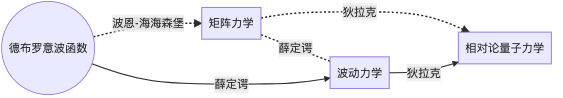
\includegraphics[width=0.9\textwidth]{figs/2021-12-06-16-22-39.png}\\   
        \end{center}    
\end{frame} 

\subsection{左矢与右矢}

\begin{frame}
    量子力学用希尔伯特空间描述,希尔伯特空间是内积空间
    \begin{tcolorbox1}{希尔伯特空间}
    \begin{itemize}
        \Item 加法:$\psi + \varphi$
        \Item 数乘:$c\psi$
        \Item 内积:$(\psi,\psi)$
    \end{itemize}
    \end{tcolorbox1}
    考察内积: $(\psi,\psi)=\int\psi^*\psi d\tau$ \\
    同一波函数放在左边还是右边,意义有所不同: \\
    放右边是线性矢量:  $(\psi,a\psi)=a (\psi,\psi)$ \\
    放左边是反线性矢量:   $(a\psi,\psi)=a^* (\psi,\psi)$   
\end{frame}

\begin{frame}
    \frametitle{左矢和右矢}
    \begin{tcolorbox1}{定义:}
    为了清楚地描述这种线性反线性特点,特定义左矢和右矢
    $$\langle \psi |, \qquad |\psi \rangle $$ 
    内积:\[(\psi,\psi)\equiv \langle \psi | \psi \rangle\]

    有性质: $$\langle a\psi | = \langle \psi |a^* $$
    $$ |a\psi \rangle = a|\psi \rangle$$ 
    \end{tcolorbox1}
\end{frame} 

\begin{frame}
    \frametitle{}
    考察加法和数乘:发现其中的矢量通常是线性的,因此用右矢来代替。\\
    $$\begin{aligned}
    &\text{内积:}   & (\psi,\Psi)  & \qquad\Leftrightarrow \qquad & | \Psi \rangle =\langle \psi | \Psi \rangle \\
    &\text{平均值:}   & \bar{F}=(\Psi,F\Psi)  & \qquad\Leftrightarrow \qquad & \bar{F} =\langle \Psi|F | \Psi \rangle \\
    &\text{态叠加原理:}   & \Psi=a_1 \psi_1+ a_2 \psi_2  & \qquad\Leftrightarrow \qquad &| \Psi \rangle =a_1 |1 \rangle+ a_2 |2 \rangle\\
    &\text{展开式1:}     & \Psi=\sum\limits_{i=1} ^n a_i \psi_i & \qquad \Leftrightarrow \qquad &| \Psi \rangle =\sum\limits_{i=1} ^n a_i |i \rangle\\
    &\text{展开式2:}     & \Psi=\sum\limits_{i=1} ^n (\psi_i ,\Psi) \psi_i & \qquad \Leftrightarrow \qquad &| \Psi \rangle =\sum\limits_{i=1} ^n \langle i | \Psi \rangle |i\rangle\\
    \end{aligned}
    $$
\end{frame} 
 
\subsection{外积}

\begin{frame}
    \frametitle{外积定义}
    考察展开式:
    $$\begin{aligned}
    \Psi \rangle &= \sum\limits_{i=1} ^n \langle i | \Psi \rangle |i\rangle\\
                 &= \sum\limits_{i=1} ^n |i\rangle\langle i | \Psi \rangle \\
    \end{aligned}
    $$
    发现存在:$|i\rangle\langle i$,称为函数的外积,有
    \[\sum\limits_{i=1} ^n |i\rangle\langle i |=1\]
    称为本征函数系的完全性(封闭性)。 
\end{frame} 

\begin{frame}
    \frametitle{}
    ~~\\
    *对于:$ \Psi =\sum a_n \varphi_n $, 这种一般态,定义:$\hat{p} = |\Psi\rangle\langle \Psi |$\\
    右矢的矩阵形式:
    $$|\Psi\rangle = \begin{pmatrix}
        a_1\\
        a_2\\\
        \cdots\\
        a_n\
    \end{pmatrix}$$ 
    左矢的矩阵形式:
    $$ \langle\Psi| = (a_1 ^*, a_2 ^*, \cdots, a_n ^*) $$
    内积与外积:
    $$\langle\Psi|\Psi\rangle= (a_1 ^*, a_2 ^*, \cdots, a_n ^*) \begin{pmatrix}
        a_1\\
        a_2\\\
        \cdots\\
        a_n\
    \end{pmatrix},\qquad  |\Psi\rangle\langle\Psi|= \begin{pmatrix}
        a_1\\
        a_2\\\
        \cdots\\
        a_n\
    \end{pmatrix} (a_1 ^*, a_2 ^*, \cdots, a_n ^*) $$
\end{frame} 

\begin{frame}
    \frametitle{密度算符}
    定义算符: $ \qquad  \hat{p}_i = |i\rangle\langle i | \qquad $ 有: 
    $$ \hat{p}_i\Psi= |i\rangle\langle i | \Psi \rangle = \langle i | \Psi \rangle |i\rangle=a_i |i\rangle $$
    $$\Psi= \sum\limits_i ^n a_i |i\rangle = \sum\limits_i ^n \hat{p}_i\Psi$$
    可知: $ \hat{p}_i\Psi $ 是矢量$\Psi$ 在第$i$ 个本征矢上的投影, 因此称为{\color{red} 投影算符}\\
    考察其在$i$态的平均值:
    $$ \begin{aligned}
    \bar{\hat{p}} &=\langle i |\hat{p} | i \rangle \\
               &=\langle i |\Psi\rangle\langle \Psi | i \rangle \\
               &=(\langle i |\Psi\rangle) (\langle \Psi | i \rangle) \\
               &=a_i ^* a_i =\omega_i \\
    \end{aligned} $$
    是概率密度,因此称 $\hat{p} = |\Psi\rangle\langle \Psi |$ 为 {\color{red} 密度算符},也称为测量算符。
\end{frame} 
 
\begin{frame}
    \frametitle{密度矩阵}
    考察平均值公式:\\
    $$ \begin{aligned}
    \bar{\hat{F}} &=\sum\limits_i |a_i|^2 f_i \\
            &=\sum\limits_i \omega_i \langle i |\hat{F}|i \rangle  \\
            &=\sum\limits_{ij} \omega_i \langle i |\hat{F} |j\rangle \langle j| i\rangle  \\
            &=\sum\limits_{ij} \langle j| i\rangle  \omega_i \langle i |\hat{F} |j\rangle  \\
            &=\sum\limits_{j} \langle j | (\sum\limits_{i}| i \rangle  \omega_i \langle i |) \hat{F} |j\rangle  \\
    \end{aligned} $$
    定义密度矩阵:$ \hat{\rho} = \sum\limits_{i}| i \rangle  \omega_i \langle i | , \qquad \hat{\rho} = \sum\limits_{i}| \Psi_i \rangle  P_i \langle \Psi_i | \quad \text{(混态)} $
\end{frame} 
 
\begin{frame}  
    \frametitle{}  得新的平均值公式:
    \begin{tcolorbox1}{平均值公式-3}
         $$ \begin{aligned}
            \bar{\hat{F}}&=\sum\limits_{j} \langle j | \hat{\rho} \hat{F} |j\rangle \\
                &=tr (\hat{\rho} \hat{F} )
        \end{aligned} $$   
    \end{tcolorbox1} 
\end{frame} 
 
\begin{frame}      
    \例[1.求算符$\hat{F}$在 $|\Psi\rangle =\sum\limits_n a_n |n\rangle $上的平均值]{}
    \解~先求算符的矩阵:
    $$ F_{nm} = \langle n | F |m \rangle  $$
    再求密度矩阵:
    $$ \hat{\rho} = \sum\limits_{n}| n \rangle  a_n ^* a_n \langle n | $$
    对两矩阵的积求迹得平均值
    $$\bar{\hat{F}}=tr (\hat{\rho} \hat{F} )$$
\end{frame} 
 
\subsection{狄拉克量子力学}

\begin{frame} 
    \frametitle{狄拉克量子力学}  
    量子态(无表象): $\hspace{1em}|\Psi \rangle, \quad$ 位置表象:$\hspace{1em} \langle x |\Psi \rangle , \quad$ 动量表象:$\hspace{1em} \langle p_x |\Psi \rangle$ \\ \vspace{0.1em}
    算符: $F, \quad$ 位置表象:$\hspace{1em} F(x, -i\hbar \frac{\partial }{\partial x}) , \quad$ 动量表象:$\hspace{1em} F(i\hbar \frac{\partial }{\partial p_x}, p_x) $ \\ \vspace{0.1em}
    展开式: $\hspace{1em}|\Psi \rangle =\sum\limits_{n=1} ^n a_n |n \rangle$ \\
    内积:   $\hspace{2em}\langle \varphi | \Psi \rangle = (\varphi, \Psi)= \int \varphi^*\Psi d\tau $ \\  \vspace{0.1em}
    归一化: $\hspace{1em}\langle \Psi | \Psi \rangle = (\Psi, \Psi)= \int \Psi^*\Psi d\tau = 1 $ \\ \vspace{0.1em}
    正交归一: $\langle n | m \rangle = \delta_{nm} $ \\ \vspace{0.1em}
    $ \hspace{5em} \langle \lambda | \lambda' \rangle = \delta(\lambda-\lambda') $\\ \vspace{0.2em}
    展开系数: $ a_n= \langle n | \Psi \rangle$ \\ \vspace{0.2em}
    展开系数: $ a_n ^*= \langle \Psi | n \rangle$ \\ \vspace{0.2em}
\end{frame} 
 
\begin{frame} 
    平均值:  $\hspace{1em}\bar{F} = \langle \Psi |F | \Psi \rangle$ \\ \vspace{0.2em}
    矩阵元:  $\hspace{1em}F_{nm} = \langle n |F | m \rangle$ \\ \vspace{0.2em}
    幺正变换:$S_{m\alpha} =\langle m| \alpha \rangle $ \\ \vspace{0.2em}
    投影算符:$p_i = |i\rangle\langle i |, \quad \text{封闭性:} \sum_i |i\rangle\langle i |=1 $ \\ \vspace{0.2em}
    密度矩阵: $\hat{\rho} = \sum\limits_{i}| i \rangle  \omega_i \langle i |, \quad \hat{\rho} = \sum\limits_{i}| \Psi_i \rangle  P_i \langle \Psi_i | $ \\ \vspace{0.2em}
    本征方程:$F|n\rangle =f_n |n\rangle$ \\ \vspace{0.2em}
    薛定谔方程:$$ i\hbar \frac{\partial }{\partial t} |\Psi(t)\rangle = H|\Psi(t)\rangle $$ 
    算符运动方程:$$ \frac{d\bar{A}(t)}{dt}=\overline{(\frac{\partial A(t) }{\partial t})}  +\frac{1}{i\hbar} \overline{[A(t),H(t)]}$$
\end{frame} 
 
\begin{frame} 
    \frametitle{应用实例}  
    1、求波函数的矩阵表示:  
    $$|\Psi \rangle =\sum\limits_{n=1} ^n a_n |n \rangle$$
    $$ a_n= \langle n | \Psi \rangle$$ 
    展开系数构成矩阵表示:  
    $$\begin{pmatrix}
    a_1\\
    a_2\\\
    \cdots\\
    a_n\
    \end{pmatrix} $$
\end{frame} 

\begin{frame} 
    \frametitle{}  
    2、求算符的矩阵表示:  
    $$|\varphi \rangle = F |\Psi \rangle$$
    $$|\varphi \rangle = \sum_n F |n\rangle\langle n |\Psi \rangle$$
    $$\langle m |\varphi \rangle = \sum_n  \langle m| F |n\rangle\langle n |\Psi \rangle$$
    $$ b_m = \sum_n  F_{mn} a_n$$

    取遍$n,m$:  
    $$\begin{pmatrix}
    b_1\\
    b_2\\\
    \cdots\\
    b_n\
    \end{pmatrix} 
    = 
    \begin{pmatrix}
        F_{11} & F_{12} & \cdots & F_{1n} \\
        F_{21} & F_{22} & \cdots & F_{2n} \\
        \cdots & \cdots &  \cdots &  \cdots \\
        F_{n1} & F_{n2} & \cdots & F_{nn} \\
    \end{pmatrix} 
    \begin{pmatrix}
        a_1\\
        a_2\\\
        \cdots\\
        a_n\
    \end{pmatrix} 
    $$
\end{frame} 

\begin{frame} 
    3、求薛定谔方程的矩阵表示: 
    $$ \begin{aligned}
    i \hbar \frac{\partial}{\partial t} |\Psi \rangle &= H |\Psi \rangle  \\
    i \hbar \frac{\partial}{\partial t} \langle m |\Psi \rangle &= \langle m |H |\Psi \rangle \\ 
     &= \sum_n \langle m |H |n\rangle\langle n |\Psi \rangle  \\
     i \hbar \frac{\partial}{\partial t} a_m  &= \sum_n H_{mn} a_n 
    \end{aligned}
    $$
\end{frame} 

\begin{frame} 
    4、求薛定谔方程在各表象中的形式: 
    $$ \begin{aligned}
    i \hbar \frac{\partial}{\partial t} |\Psi(t) \rangle &= H |\Psi(t) \rangle  , \quad \text{无表象}\\
    i \hbar \frac{\partial}{\partial t} \langle x|\Psi(t) \rangle &= H (x, \hat{p}_x) \langle x|\Psi(t) \rangle  , \quad \text{位置表象}\\
    i \hbar \frac{\partial}{\partial t} \langle x|\Psi(t) \rangle &= [- \frac{\hbar^2}{2\mu} \frac{\partial ^2 }{\partial x^2} + U(x)] \langle x|\Psi(t) \rangle  , \quad \text{位置表象}\\
    i \hbar \frac{\partial}{\partial t} \langle p_x|\Psi(t) \rangle &= H (\hat{x}, p_x) \langle p_x|\Psi(t) \rangle  , \quad \text{动量表象}\\
    i \hbar \frac{\partial}{\partial t} \langle p_x|\Psi(t) \rangle &=  [ \frac{p^2 _x}{2\mu} + U(i \hbar \frac{\partial }{\partial p_x}) ] \langle p_x|\Psi(t) \rangle  , \quad \text{动量表象}\\
    i \hbar \frac{\partial}{\partial t} \langle n|\Psi(t) \rangle &=  \langle n|H|m \rangle \langle n |\Psi(t) \rangle  , \quad \text{Q表象}\\
    \end{aligned}
    $$
\end{frame} 

\begin{frame} 
    5、求平均值公式的矩阵表示: 
    $$ \begin{aligned}
    \bar{F} &= \langle \Psi |F |\Psi \rangle  \\
    &= \langle \Psi |1 \cdot F \cdot 1 |\Psi \rangle  \\
    &= \sum_{mn} \langle \Psi |m\rangle\langle m |F| n\rangle\langle n |\Psi \rangle  \\
    &= \sum_{mn} a_m ^* F_{mn} a_n 
    \end{aligned}
    $$
\end{frame} 

\begin{frame} 
    6、求两算符积的平均值公式的矩阵表示: 
    $$ \begin{aligned}
    \overline{GF} &= \langle \Psi |GF |\Psi \rangle  \\
    &= \langle \Psi |1 \cdot G \cdot 1 \cdot F \cdot 1 |\Psi \rangle  \\
    &= \sum_{mln} \langle \Psi |m\rangle\langle m |G |l\rangle\langle l| F| n\rangle\langle n |\Psi \rangle  \\
    &= \sum_{mln} a_m ^* G_{ml} F_{ln} a_n 
    \end{aligned}
    $$
\end{frame} 

\begin{frame} 
    \frametitle{课堂作业}
    设体系处于叠加态 $\rs{\psi}=\State$, 现定义如下算符
    \[F= \ls{0}{1}+\ls{1}{0}\]
    求$F\rs{\psi}=?$  
\end{frame} 

\section{4.量子力学绘景(Pictures)}

\begin{frame}  
    \frametitle{三种绘景}
    量子力学的二个基本方程:  
    \begin{enumerate}
        \Item 薛定谔方程:$$ i\hbar \frac{\partial }{\partial t} |\Psi(t)\rangle = H|\Psi(t)\rangle $$
        \Item 算符运动方程:$$ \frac{d\bar{A}(t)}{dt}=\overline{(\frac{\partial A(t) }{\partial t})}  +\frac{1}{i\hbar} \overline{[A(t),H(t)]}$$
    \end{enumerate}
    这个世界到底什么在变?\\
    \begin{itemize}
        \done 薛定谔绘景:只有波函数(态)在变,服从薛定谔方程
        \done 海森堡绘景:只有算符(力学量)在变,服从算符运动方程(海森堡方程)
        \done 狄拉克绘景:波函数和算符都在变,一切都只是幺正变换。
    \end{itemize}
\end{frame} 

\begin{frame}  
    \frametitle{}  
    定义时间演化算符:
    $$ U(t,t_0) |\Psi(t_0)\rangle = |\Psi(t)\rangle  $$
    \alert{分析}:
    (1) 因为 $ U(t_0,t_0) |\Psi(t_0)\rangle = |\Psi(t_0)\rangle  $ \\
     有:$$ U(t_0,t_0)=I $$
    (2):求 $ U(t,t_0)$
    $$ \begin{aligned}
        i\hbar \frac{\partial }{\partial t} |\Psi(t)\rangle &= H|\Psi(t)\rangle  \\
        i\hbar \frac{\partial }{\partial t}  U(t,t_0) |\Psi(t)\rangle &= H U(t,t_0) |\Psi(t)\rangle  \\
        i\hbar \frac{\partial }{\partial t}  U(t,t_0)  &= H U(t,t_0)  \\
        U(t,t_0)  &= e^{-\frac{i}{\hbar} H(t-t_0)}  \\
    \end{aligned} $$
\end{frame} 

\begin{frame}  
    (3):$ U(t,t_0)$是幺正算符
    $$ \begin{aligned}
        U(t,t_0)  &= e^{-\frac{i}{\hbar} H(t-t_0)}  \\
        U^\dagger (t,t_0)  &= e^{\frac{i}{\hbar} H(t-t_0)}  \\
        U^\dagger (t,t_0)U(t,t_0) &= U^\dagger (t,t_0)U(t,t_0) \\
         &=e^{\frac{i}{\hbar} H(t-t_0)-\frac{i}{\hbar} H(t-t_0)} \\
         &=e^0=I
    \end{aligned} $$
    因此,有:
    $$ |\Psi(t)\rangle = U(t,t_0) |\Psi(t_0)\rangle   $$
    对比: 
    $$ |\psi_{(B)}\rangle = S^\dagger |\psi_{(A)}\rangle $$
    \Note ~波函数随时间的演化服从的薛定谔方程,只是一种幺正变换。
\end{frame} 

\begin{frame}  
    \frametitle{} 
    (4)分析平均值公式:
    $$ \begin{aligned}
        \bar{F} &= \langle \Psi(t) |F(t_0) | \Psi \rangle(t)  \\
        &= \langle \Psi(t_0) |U^\dagger (t,t_0) |F(t_0) | U(t,t_0) |\Psi(t_0)\rangle   \\
        &= \langle \Psi(t_0) |U^\dagger (t,t_0) F(t_0) U(t,t_0) |\Psi(t_0)\rangle   \\
        &= \langle \Psi(t_0) F(t,t_0) |\Psi(t_0)\rangle   \\
    \end{aligned} $$
     式中,令: $$ F(t,t_0) =U^\dagger (t,t_0) F(t_0) U(t,t_0)$$
     对式:
     $$F'=S^\dagger F S $$
     \Note ~算符随时间的演化与波函数随时间的演化是等价的,他们都是幺正变换。
\end{frame} 

\begin{frame}
      \frametitle{世界的变化}
        \begin{center}
             
\includegraphics[width=0.8\textwidth]{figs/2022-04-10-10-07-10.png}
        \end{center}   
        \begin{quotation}
            "我们必须把科学当艺术,然后才能从科学中得到完整的知识"  \\
            \rightline{$\cdots$ [德国]~ 歌德 \hspace{3em}}   
        \end{quotation}  
\end{frame}
%%%%%%%%%%%%%%%%%%%%%%%%%%%%%%%%%%%%%%%%%%%%%%%%%%%%%%%%%%%%%%%%%%%
\begin{frame}
    \frametitle{课外作业}
    \begin{enumerate}
        \item 试证明 对于任意态$\ls{\varphi}$, 若有$\lr{\varphi}{\Psi}=\lr{\varphi}{\psi} $,则$ \rs{\Psi}=\rs{\psi}$ 
        \item 基于位置算符的本征矢定义算符$\rho=\rs{x}{x}$, 试对任意态计算$\lcr{\psi}{\rho}{\psi}$
        \item 试证明在幺正变换下两个态的内积保持不变.
        \item 试证明在幺正变换下算符的本征值保持不变.
        \item 试写出定态薛定谔方程和平均值公式在动量表象和Q表象中的具体形式 (Dirac):
        \item 设氢原子处于$\rs{\psi}=0.5Y_{11}+0.4Y_{20}$态 ,试求 $L_x$,$L_y$的可能值,取值概率及平均值 
    \end{enumerate}
\end{frame}
%%%%%%%%%%%%%%%%%%%%%%%%%%%%%%%%%%%%%%%%%%%%%%%%%%%%%%%%%%%%%%%%%%%
\begin{frame}
    \frametitle{}  
    \centering
    \LARGE \color{red} 期中考试! \\
\end{frame}